\ac{THOR} currently includes two tutorials to guide new users through the process of creating a mesh with Gmsh, using OpenMeshConverter to make it a \ac{THOR} mesh, and running \ac{THOR} using that mesh.
The first tutorial is the Godiva tutorial, creating a model of the bare Godiva critical experiment sphere, meshing it, and running it with \ac{THOR}.
This tutorial demonstrates basic \ac{THOR} problem creation and running concepts.

The second tutorial is the BeRP tutorial, creating a model of the BeRP ball with 3 inches of polyethylene reflector surrounding the BeRP ball.
This tutorial demonstrates a more advanced problem involving multiple materials and regions.
Additionally this is a fixed source problem used to demonstrate the fixed source capabilities of the THOR transport solver.

Since both systems are physically equivalent to one-dimensional spherical problems, the symmetry is taken advantage of and the problems are modeled using a one/eighth model with reflective boundary conditions to be equivalent to the full spheres for the tutorial.
In the tutorial folders, \\
\verb"<thor_dir>/THOR/examples/Godiva_tutorial" and \verb"<thor_dir>/THOR/examples/BeRP_tutorial", versions of these tutorials with full spheres, half spheres, and quarter spheres are also included along with reference results.

\section{Godiva Tutorial}

Godiva is an un-shielded, pulsed, nuclear burst reactor. It is essentially a homogeneous sphere of highly enriched uranium with a diameter of $30$ cm, that was operated by inserting a piston of fissile material~\cite{Godiva1961}.
In this tutorial the critical benchmark configuration described in Ref.~\cite{GodivaBenchmark} is considered. The geometry that is modeled by \ac{THOR} is a homogeneous sphere of radius $8.7407$ cm discretized by tetrahedra similar to Fig.~\ref{fig:godiva_coarse}.
The energy domain is discretized with six energy groups, and cross sections are provided by~\cite{GodivaBenchmark}.

\begin{figure}[th]
  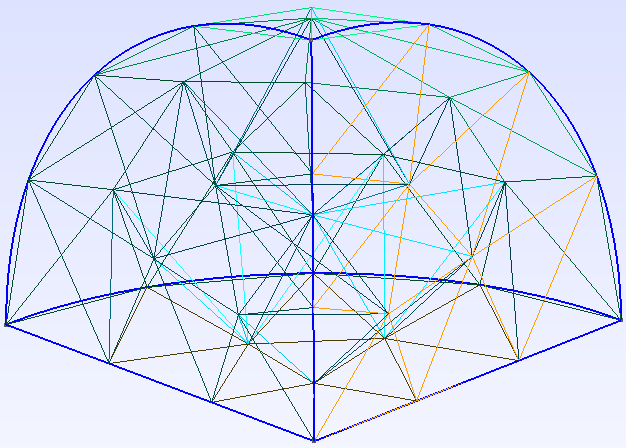
\includegraphics[width=1.0\textwidth]{chapters/tutorials/figures/godiva_coarse.png}
  \caption{Coarse mesh for Godiva problem}
  \label{fig:godiva_coarse}
\end{figure}

This tutorial first explains how a tetrahedral mesh is created for the Godiva problem, then the cross sections data input is discussed, and finally the standard input to \ac{THOR} is covered.
The input files discussed below for the Godiva tutorial are located in:
\begin{verbatim}
    >> <thor_dir>/THOR/examples/Godiva_tutorial
\end{verbatim}

\subsection{Godiva Mesh}\label{ch:tuts:sec:godiva:ssec:mesh}

The workflow described here is suitable if the user has access to a compatible version of \href{https://gmsh.info/}{Gmsh}.
Any version 4 Gmsh should work, but the example specifically performed here was done using Gmsh version 4.10.1.

Begin by navigating to the location of the Godiva Gmsh geometry files, which are found in:
\begin{verbatim}
  <thor_dir>/THOR/examples/Godiva_tutorial/mesh_create/
\end{verbatim}
Opening the file geometry file \verb"godiva_octant.geo" in a text editor, it can be observed that the model is created by removing the negative portions of each direction from a sphere centered at the origin.
For more details on creating original Gmsh inputs, see the \href{https://gmsh.info/doc/texinfo/gmsh.html}{Gmsh reference manual}.

Open \verb"godiva_octant.geo" in Gmsh and run the ``3D'' command from the ``Mesh'' dropdown menu under ``Modules''.
The mesh should be generated and now become visible in the \ac{GUI}.
Now, select the ``Save'' command from the same ``Mesh'' dropdown to save the generated mesh to \verb"godiva_octant.msh".
This mesh may be compared to the provided \verb"godiva_octant_msh.ref", however they may differ slightly if the versions differ or if optimization of the mesh is employed.

The gmsh file \verb"godiva_octant.msh" is converted to \ac{THOR}'s native mesh format by executing OpenMeshConverter with the command line:
\begin{verbatim}
  >> <thor_dir>/THOR/pre-processors/OpenMeshConverter/OpenMeshConverter.exe
      convert_godiva.msh -bc 1 0 1 0 1 0
\end{verbatim}
Note that since we are modeling the fully positive octant of the sphere we are setting all of the flat negative faces to be reflective (see Section~\ref{ch:getstart:sec:preproc:subsec:meshconv} for more details).
After successful completion of the conversion, the following printout should appear:
\begin{verbatim}
----------------------- Reading in gmsh:
Progress:***********************************************************************
----------------------- Calculating Adjacencies:
Progress:***********************************************************************
----------------------- Outputting thrm file:
Progress:***********************************************************************
----------------------- Calculating volumes:
Progress:***********************************************************************
Region 5 volume:   3.3099604624050352E+02
Region 5 equivalent radius:   4.2911933629822876E+00
Total system volume:   3.3099604624050352E+02
Equivalent radius:   4.2911933629822876E+00
--------------------------------------------------------------------------------
--------------------------------------------------------------------------------
--------------------------------------------------------------------------------
------------------------- OpenMeshConverter successful -------------------------
----------------------- Output written to godiva_octant.thrm
\end{verbatim}

The file \verb"godiva_octant.thrm" should result from this execution for use by THOR.
This mesh may be compared to the provided \verb"godiva_octant_thrm.ref", which it should match if \verb"godiva_octant.msh" matches \verb"godiva_octant_msh.ref".
Notice that the given volume for Region 5 (the Godiva eighth of a sphere as seen in \verb"godiva_octant.geo") is 330.996~cm$^3$, but the actual octant volume for the Godiva sphere is 349.653~cm$^3$.
The ratio of the actual volume to the meshed volume is then 1.056366, which will come in handy later.
This concludes the mesh generation step for this tutorial.

\subsection{Cross section data}

The user should now move \verb"godiva_octant.thrm" to the input file location
\begin{verbatim}
  <thor_dir>/THOR/examples/Godiva_tutorial/
\end{verbatim}
and navigate there to continue the tutorial.

The \ac{THOR} cross section file for the Godiva benchmark is provided by \verb"godiva.xs".
\ac{THOR} uses a custom cross section format that is explained in detail in Section~\ref{ch:inp:sec:xsfile}.

At the end of Section~\ref{ch:tuts:sec:godiva:ssec:mesh}, it was observed that there was a discrepancy in the volume of the Godiva mesh compared to the original problem.
To preserve material mass, the cross sections must be altered by increasing them by a factor of 1.056366.
In \ac{THOR}, the user need not alter the cross sections themselves to make this adjustment.
Instead, \ac{THOR} will automatically adjust reaction and material attenuation calculations by a given density factor for each region.
By default, this factor is 1.0, which will lead to use of the original cross sections unaltered.
However, the user may specify density factors in a density factor file, described in Section~\ref{ch:inp:sec:densfact}.
For this tutorial, this density factor adjustment is provided by \verb"godiva_octant.dens"

\subsection{THOR input file and executing THOR}

The \ac{THOR} input file is \verb"godiva_octant.inp".
\ac{THOR} uses a keyword-based input that is listed in Section~\ref{ch:inp:sec:stdinput}.
The Godiva tutorial input file is verbose and some parameters are ignored as they are not relevant to the problem.
Upon running \ac{THOR}, a verbose form of the input will always be echoed, and ignored parameters will be highlighted as such.
\begin{verbatim}
problem_type          keig
keigsolver            pi
lambda                0
inflow                no
piacc                 errmode
page_sweep            no
page_refl             save
page_iflw             all
kconv                 1e-8
innerconv             1e-12
outerconv             1e-7
maxinner              4
maxouter              5000
jfnk_krsze            25
jfnk_maxkr            250
jfnk_method           flat
initial_guess         no
restart_out           no
ipiter                0
print_conv            yes
density_factor        godiva_octant.dens
execution             yes
mesh                  ./godiva_octant.thrm
source                source.dat
flux_out              no
xs                    ./godiva.xs
vtk_flux_out          yes
vtk_mat_out           yes
vtk_reg_out           no
vtk_src_out           no
cartesian_map_out     no
print_xs              no
ngroups               1
pnorder               0
pnread                0
upscattering          yes
multiplying           yes
scatt_mult_included   yes
qdtype                levelsym
qdorder               4
cartesian_map         no
point_value_locations no
region_map            5 1
\end{verbatim}

The Godiva tutorial is solved with \ac{THOR} via the command line:
\begin{verbatim}
  >> <thor_dir>/THOR/thor-1.0.exe godiva_octant.inp
\end{verbatim}

Completion of execution of the Godiva tutorial is indicated by the printout:
\begin{verbatim}
--------------------------------------------------------
   Execution of THOR completed successfully
--------------------------------------------------------
\end{verbatim}

\ac{THOR} provides the following output that is discussed in this tutorial:
\begin{itemize}
    \item The final estimate of the multiplication factor is printed under ``Execution Summary'', ``Final eigenvalue''.
    In this case the value is $0.935$. This is not close to critical because the mesh that
    is created is very coarse.
    \item A summary of group-wise, region-averaged reaction rates is provided for each region identifier separately under ``Region averaged reaction rates''.
    The volume of each region, and group-wise fluxes, fission, absorption, and fission source rates are listed.
    \item Two vtk formatted files, \verb"godiva_octant_flux.vtk" contains spatial flux maps, and \\
    \verb"godiva_octant_mat.vtk" contains the material map. These files can be opened with the \href{https://www.paraview.org/download/}{ParaView} post-processing tool.
\end{itemize}

A plot of the fast flux using ParaView 5.10.0 for this run is shown in Figure~\ref{fig:godiva_fast}.
\begin{figure}[th]
  \center
  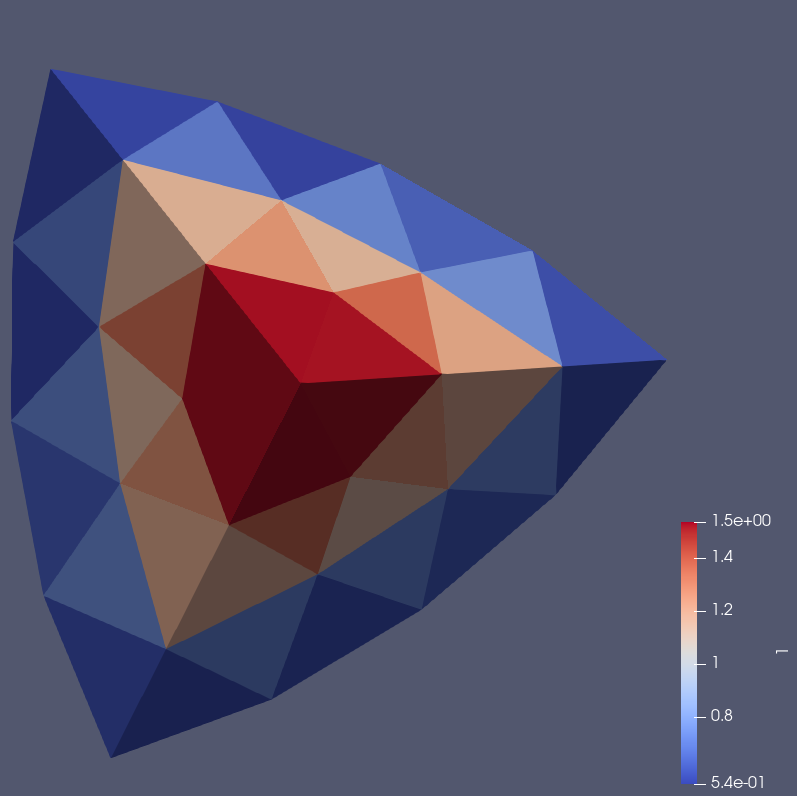
\includegraphics[height=0.5\textwidth]{chapters/tutorials/figures/godiva_fast.png}
  \caption{Fast flux for Godiva tutorial.}
  \label{fig:godiva_fast}
\end{figure}

The reaction rate summary is given by:
\begin{verbatim}
--------------------------------------------------------
   Region averaged reaction rates
--------------------------------------------------------

-- Region --   5 -- Material -- mat_1 Volume =   3.309960E+02
   Group          Flux       Fission    Absorption      Fiss Src
       1  8.317355E-01  1.381271E-01  4.883317E-02  1.381271E-01
       2  1.549185E+00  2.298278E-01  9.364997E-02  2.298278E-01
       3  9.627054E-01  1.353285E-01  5.854598E-02  1.353285E-01
       4  1.585196E+00  2.152633E-01  9.782396E-02  2.152633E-01
       5  1.137791E+00  1.819135E-01  8.630310E-02  1.819135E-01
       6  1.682607E-01  4.366399E-02  2.265428E-02  4.366399E-02
   Total  6.234875E+00  9.441242E-01  4.078105E-01  9.441242E-01
\end{verbatim}

The results can be improved by increasing the refinement of the mesh.
This can be achieved by reducing the mesh size parameter in the \verb"godiva_octant.geo" file, that parameter is \\
\verb"MeshSize{ PointsOf{ Volume{:}; } };" which can be seen is set to 4.

\section{Polyethylene Shielded BeRP Ball Tutorial}

The BeRP ball is a weapons grade plutonium sphere used in detector and criticality experiments~\cite{BeRP_report}.
The ball represents a fission neutron source that is subcritical under normal conditions.
The sphere has a mean radius of 3.7938~cm.
The calculated density of the sphere is 19.604 g/cm$^3$ giving the plutonium a total mass of 4,483.884 g.

The BeRP ball is designed to be inserted into reflecting spherical shells.
These shells act as both a moderating reflector that increases the induced fission rate produced in the ball, as well as a shield changing the spectrum and strength of the emitted neutrons that escape the reflector.
The shells exist in a variety of sizes, with larger shells fitting around smaller shells to go from at least 0.5 inches to up to at least 6 inches.
Shells also exist in a variety of materials including but not limited to \ac{HDPE} and copper.

This tutorial includes the 3 inch polyethylene shield as the shell for the BeRP ball.

\begin{figure}[th]
  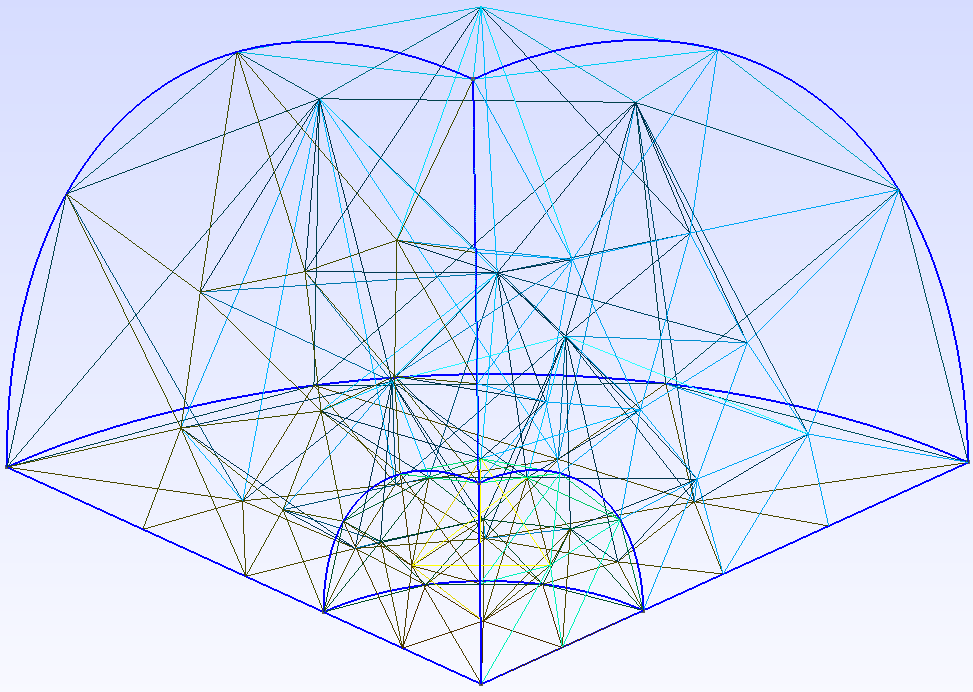
\includegraphics[width=1.0\textwidth]{chapters/tutorials/figures/berp_coarse.png}
  \caption{Coarse mesh for BeRP Ball with Poly Shield}
  \label{fig:berp_coarse}
\end{figure}

This tutorial first explains how a tetrahedral mesh is created for the BeRP ball surrounded by a poly shield, then the cross sections data input is discussed, the source specification is discussed, and finally the standard input to THOR is covered.
The input files discussed below for the BeRP tutorial are located in:
\begin{verbatim}
    >> <thor_dir>/THOR/examples/BeRP_tutorial
\end{verbatim}

\subsection{BeRP Ball Mesh}\label{ch:tuts:sec:berp:ssec:mesh}

The workflow described here is suitable if the user has access to a compatible version of \href{https://gmsh.info/}{Gmsh}.
Any version 4 Gmsh should work, but the example specifically performed here was done using Gmsh version 4.10.1.

Begin by navigating to the location of the BeRP Gmsh geometry files, which are found in:
\begin{verbatim}
  <thor_dir>/THOR/examples/BeRP_tutorial/mesh_create/
\end{verbatim}
Opening the file geometry file \verb"berp_octant.geo" in a text editor, it can be observed that the model is created by removing the negative portions of each direction from a sphere centered at the origin surrounded by another sphere centered at the origin.
For more details on creating original Gmsh inputs, see the \href{https://gmsh.info/doc/texinfo/gmsh.html}{Gmsh reference manual}.

Open \verb"berp_octant.geo" in Gmsh and run the ``3D'' command from the ``Mesh'' dropdown menu under ``Modules''.
The mesh should be generated and now become visible in the \ac{GUI}.
Now, select the ``Save'' command from the same ``Mesh'' dropdown to save the generated mesh to \verb"berp_octant.msh".
This mesh may be compared to the provided \verb"berp_octant_msh.ref", however they may differ slightly if the versions differ or if optimization of the mesh is employed.

The gmsh file \verb"berp_octant.msh" is converted to \ac{THOR}'s native mesh format by executing OpenMeshConverter with the command line:
\begin{verbatim}
  >> <thor_dir>/THOR/pre-processors/OpenMeshConverter/OpenMeshConverter.exe
      berp_octant.msh -bc 1 0 1 0 1 0
\end{verbatim}
Note that since we are modeling the fully positive octant of the sphere we are setting all of the flat negative faces to be reflective (see Section~\ref{ch:getstart:sec:preproc:subsec:meshconv} for more details).
After successful completion of the conversion, the following printout should appear:
\begin{verbatim}
----------------------- Reading in gmsh:
Progress:***********************************************************************
----------------------- Calculating Adjacencies:
Progress:***********************************************************************
----------------------- Outputting thrm file:
Progress:***********************************************************************
----------------------- Calculating volumes:
Progress:***********************************************************************
Region 1 volume:   2.6511347836966994E+01
Region 1 equivalent radius:   1.8497558414045954E+00
Region 2 volume:   6.6374040817476271E+02
Region 2 equivalent radius:   5.4113202652319341E+00
Total system volume:   6.9025175601172975E+02
Equivalent radius:   5.4824287000562011E+00
--------------------------------------------------------------------------------
--------------------------------------------------------------------------------
--------------------------------------------------------------------------------
------------------------- OpenMeshConverter successful -------------------------
----------------------- Output written to berp_octant.thrm
\end{verbatim}

The file \verb"berp_octant.thrm" should result from this execution for use by \ac{THOR}.
This mesh may be compared to the provided \verb"berp_octant_thrm.ref", which it should match if \verb"berp_octant.msh" matches \verb"berp_octant_msh.ref".
Notice that the given volume for Region 6 (the BeRP eighth of a sphere as seen in \verb"berp_octant.geo") is 26.511~cm$^3$, but the actual octant volume for the BeRP ball is 28.591~cm$^3$.
Similarly, the given volume for Region 7 (the Poly shield eighth of a sphere as seen in \verb"berp_octant.geo") is 663.740~cm$^3$, but the actual octant volume for the Poly shield is 749.965~cm$^3$.
The ratio of the actual volume to the meshed volume for these two regions is then 1.078425 and 1.129907 respectively, which will come in handy later.
This concludes the mesh generation step for this tutorial.

\subsection{Cross section data}

The user should now move \verb"berp_octant.thrm" to the input file location
\begin{verbatim}
  <thor_dir>/THOR/examples/BeRP_tutorial/
\end{verbatim}
and navigate there to continue the tutorial.

The \ac{THOR} cross section file for the BeRP benchmark is provided by \verb"berp.xs".
\ac{THOR} uses a custom cross section format that is explained in detail in Section~\ref{ch:inp:sec:xsfile}.

At the end of Section~\ref{ch:tuts:sec:berp:ssec:mesh}, it was observed that there was a discrepancy in the volume of the BeRP mesh compared to the original problem.
To preserve material mass, the cross sections must be altered by increasing them by a factor of 1.078425 in the BeRP ball and 1.129907 in the polyethylene.
In \ac{THOR}, the user need not alter the cross sections themselves to make this adjustment.
Instead, \ac{THOR} will automatically adjust reaction and material attenuation calculations by a given density factor for each region.
By default, this factor is 1.0, which will lead to use of the original cross sections unaltered.
However, the user may specify density factors in a density factor file, described in Section~\ref{ch:inp:sec:densfact}.
For this tutorial, this density factor adjustment is provided by \verb"berp_octant.dens".
This file differs from the file in the Godiva tutorial in that it gives true region volumes instead of ratios of true to meshed volumes.
The effect is the same, however it is often simpler to specify the density factors in this manner since the density file will then need not be changed as the mesh is refined.

\subsection{Source specification}

The \ac{THOR} source file for the BeRP benchmark is provided by \verb"berp.src".
\ac{THOR} uses a custom source format that is explained in detail in Section~\ref{ch:inp:sec:srcfile}.
Notice that mapping for source regions is not done (unlike cross section mapping), so the sources must be assigned to the proper source region in the source file compared to the THOR mesh.
For this problem that simply means source region 1 must be assigned all of the spontaneous fission source since OpenMeshConverter automatically assigns each cell matching region and source IDs, which for the BeRP spehere is region 1 as seen in \verb"berp_octant.geo".

\subsection{THOR input file and executing THOR}

The \ac{THOR} input file is \verb"berp_octant.inp".
\ac{THOR} uses a keyword-based input that is listed in Section~\ref{ch:inp:sec:stdinput}.
The BeRP tutorial input file is not verbose and all parameters given are used, though not all are necessary since many are the same as the default values.
Upon running \ac{THOR}, a verbose form of the input will always be echoed, and ignored parameters will be highlighted as such.
\begin{verbatim}
  print_conv yes
  lambda 0
  problem_type fsrc ; piacc errmode
  page_refl save
  innerconv 1E-8 ; outerconv 1E-6
  maxinner 5 ; maxouter 5000

  mesh ./berp_octant.thrm
  xs ./berp.xs
  source ./berp.src
  density_factor berp_octant.dens
  vtk_flux_out yes
  vtk_mat_out yes
  vtk_src_out yes

  qdtype levelsym ; qdorder 4

  region_map
  1 1
  2 2
\end{verbatim}

The BeRP tutorial is solved with \ac{THOR} via the command line:
\begin{verbatim}
  >> <thor_dir>/THOR/thor-1.0.exe berp_octant.inp
\end{verbatim}

Completion of execution of the BeRP tutorial is indicated by the printout:
\begin{verbatim}
--------------------------------------------------------
   Execution of THOR completed successfully
--------------------------------------------------------
\end{verbatim}

\ac{THOR} provides the following output that is discussed in this tutorial:
\begin{itemize}
    \item A summary of group-wise, region-averaged reaction rates is provided for each region identifier separately under ``Region averaged reaction rates''.
    The volume of each region, and group-wise fluxes, fission, absorption, and fission source rates are listed.
    \item Three vtk formatted files, \verb"berp_octant_flux.vtk" contains spatial flux maps, \\
    \verb"berp_octant_mat.vtk" contains the material map, and \verb"berp_octant_src.vtk" contains the specified external source.
    These files can be opened with the \href{https://www.paraview.org/download/}{ParaView} post-processing tool.
\end{itemize}

A plot of the thermal flux using ParaView 5.10.0 for this run is shown in Figure~\ref{fig:berp_thermal}.
\begin{figure}[th]
  \center
  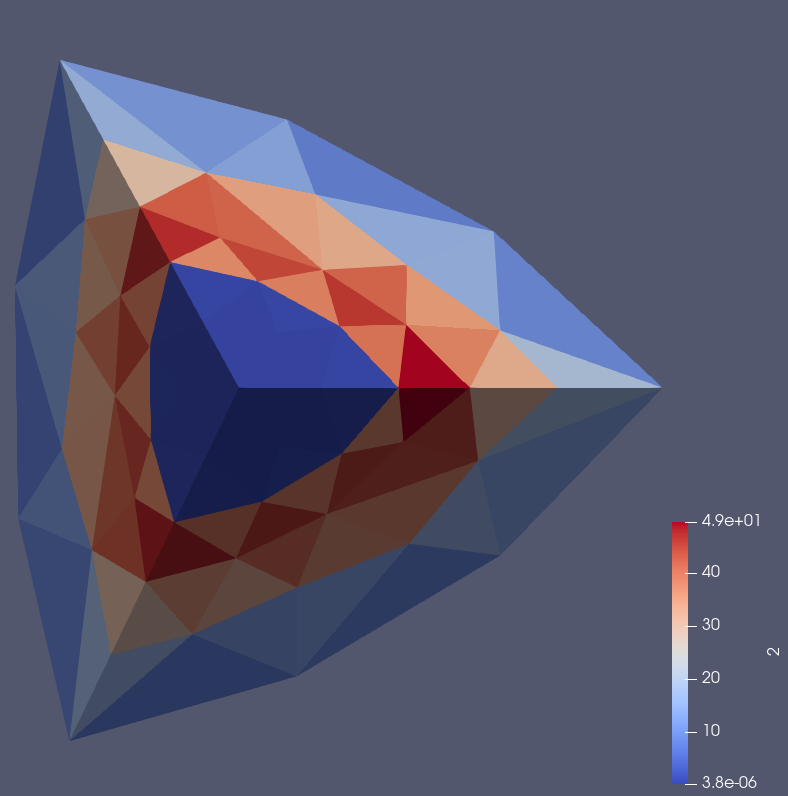
\includegraphics[height=0.5\textwidth]{chapters/tutorials/figures/berp_thermal.png}
  \caption{Thermal flux for BeRP tutorial.}
  \label{fig:berp_thermal}
\end{figure}

The reaction rate summary is given by:
\begin{verbatim}
--------------------------------------------------------
   Region averaged reaction rates
--------------------------------------------------------

-- Region --   1 -- Material -- plutonium Volume =   2.651135E+01
   Group          Flux       Fission    Absorption      Fiss Src
       1  5.196490E+00  4.707251E-01  1.136720E+00  1.472595E+00
       2  1.081906E-04  2.850034E-03  4.192962E-03  8.191729E-03
   Total  5.196598E+00  4.735752E-01  1.140913E+00  1.480786E+00

-- Region --   2 -- Material -- poly Volume =   6.637404E+02
   Group          Flux       Fission    Absorption      Fiss Src
       1  3.435603E-01  0.000000E+00  1.993624E-02  0.000000E+00
       2  8.079340E-03  0.000000E+00  1.166605E-03  0.000000E+00
   Total  3.516397E-01  0.000000E+00  2.110285E-02  0.000000E+00
\end{verbatim}

The results can be improved by increasing the refinement of the mesh.
This can be achieved by reducing the mesh size parameter in the \verb"berp_octant.geo" file, that parameter is \\
\verb"MeshSize{ PointsOf{ Volume{:}; } };" which can be seen is set to 6 for the poly and 2 for the BeRP.